\documentclass{../cssheet}

%--------------------------------------------------------------------------------------------------------------
% Basic meta data
%--------------------------------------------------------------------------------------------------------------

\title{Ähnlichkeit -- Präsenzaufgaben}
\author{Prof. Dr. Christian Spannagel}
\date{\today}
\hypersetup{%
    pdfauthor={\theauthor},%
    pdftitle={\thetitle},%
    pdfsubject={Aufgabenblatt Inside Math!},%
    pdfkeywords={insidemath,aehnlichkeit,geometrie}
}

%--------------------------------------------------------------------------------------------------------------
% document
%--------------------------------------------------------------------------------------------------------------

\begin{document}
\printtitle

\vspace*{5mm}

\textbf{Aufgabe 1 (Gewichtsvergleich):}  Max ist 1,60~m groß und wiegt 50~kg. Noah ist 2~m groß und hat eine ähnliche Statur. Wie viel wiegt Noah ungefähr?

%% ungefähr das Doppelte (100kg)

\textbf{Aufgabe 2 (Hai-Alarm):}  Taucher*innen berichten manchmal, dass sie einen gigantisch großen Hai gesehen haben. Dazu muss man wissen, dass durch eine Taucherbrille Objekte unter Wasser vergrößert erscheinen. Ein 1,2~m langer Hai erscheint unter Wasser 1,6~m lang zu sein. Welche Auswirkungen hat dies auf die wahrgenommene Körpermasse des Hais?
% (4/3)^3 = 2,4 => 240%

\textbf{Aufgabe 3 (Tetra-Paks):} Ein Getränk kommt in Packungen der Größe 0,25~l und 0,5~l auf den Markt. Wie viel mehr Verpackungsmaterial braucht man für die große Packung?
% 59% mehr Verpackungsmaterial; erst k ausrechnen (1,26) und dann quadrieren

\textbf{Aufgabe 4 (Schokohasen):} An Ostern gibt es Schokohasen unterschiedlicher Größe. Große Hasen wiegen doppelt so viel wie kleine  Hasen. Wie viel höher sind die großen Hasen als die kleinen Hasen? (Hinweis: Die Hasen sind innen hohl, die Schokolade ist bei allen Hasen gleich dick).
% Wurzel aus 2 (Diesmal spielt - obwohl Gewicht - nur die Oberfläche die entscheidende Rolle)

\textbf{Aufgabe 5 (Komische Kopierer):} Wenn man bei einem Fotokopierer von DIN~A4 auf DIN~A5 verkleinern will, dann wird als
Änderungsungsfaktor der Wert 71\% angegeben. Weshalb eigentlich? Was hättest du als Faktor vermutet? Begründe!
\begin{center}
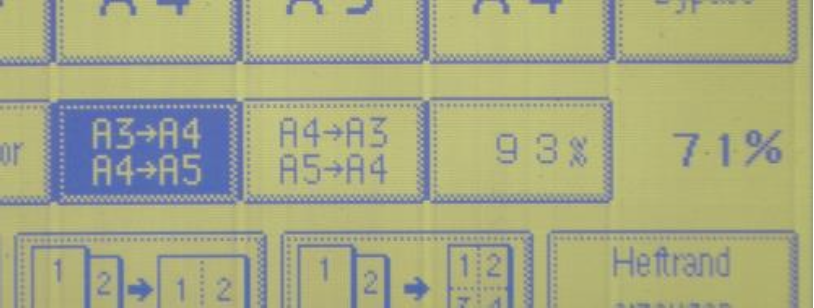
\includegraphics[width=6cm]{kopierer.png}
\end{center}

Einige Aufgaben sind entlehnt an Glaeser, G. (2008). \emph{Der mathematische Werkzeugkasten. Anwendungen in Natur und Technik (3.~Aufl.)}. Heidelberg: Spektrum Akademischer Verlag.

\vspace*{10mm}
\printlicense

\printsocials


\end{document}
